\section{\SecMapprojectionSetting} \label{subsec:adv_mapproj}
%------------------------------------------------------
\scalerm では、格子点は実距離に基づいて配置される。
各格子点での緯度・経度の値は、基準位置の緯度経度を与えることによって、ある地図投影法から計算される。
格子の緯度・経度に関する情報は、SCALE が生成するNetCDF形式の全出力ファイルに含まれる。
計算領域の位置と地図投影法は、\nmitem{PARAM_MAPPROJECTION}で設定できる。
この設定は、\textcolor{blue}{\texttt{pp.conf}、\texttt{init.conf}、\texttt{run.conf}の設定ファイル間で一致させなければならない}。
上記の設定例を以下に示す。
\editboxtwo{
\verb|&PARAM_MAPPROJECTION| & \\
\verb| MAPPROJECTION_basepoint_lon = 138.727778D0,| & \\
\verb| MAPPROJECTION_basepoint_lat = 35.360556D0,|  & \\
\verb| MAPPROJECTION_type          = 'MER',|        & ; 表\ref{tab:map_proj}から選択.\\
\verb|/| & \\
}

\begin{table}[h]
\begin{center}
\caption{\scalerm で選択可能な地図投影法}
\begin{tabularx}{150mm}{|l|X|} \hline
 \rowcolor[gray]{0.9} \verb|MPRJ_type| & 地図投影法 \\ \hline
 \verb|NONE| & 地図投影なし(理想実験用)、デフォルト \\ \hline
 \verb|LC|   & ランベルト正角円錐図法              \\ \hline
 \verb|PS|   & ポーラーステレオ図法                \\ \hline
 \verb|MER|  & メルカトル図法                     \\ \hline
 \verb|EC|   & 正距円筒図法                       \\ \hline
\end{tabularx}
\label{tab:map_proj}
\end{center}
\end{table}

\noindent
\nmitem{MPRJ_basepoint_lat, MPRJ_basepoint_lon}は、
それぞれ基準点の緯度・経度である。
デフォルトの設定では、基準点は計算領域の中心である。
\scalerm では、北緯を正、南緯を負の値として表現し、
東経を正、西経を負の値として表現する。
経度は180度以上の値を用いて表現することができる。
上記の設定では、計算領域の中心が北緯35.360556度、東経138.727778度に設定されている。
計算領域の全体は、指定された大きさでこの場所を中心にして配置される。

\nmitem{MAPPROJECTION_type}は地図投影法の種類を表しており、\verb|MER|はメルカトル図法を意味する。
表\ref{tab:map_proj}は、\scalerm で現在選択できる地図投影法を示している。
メルカトル図法の場合には、投射する円筒に接する基準緯線を\nmitem{MAPPROJECTION_M_lat}で設定する(単位は度)。
一般的に基準緯線は赤道にとることが多い。
しかし、メルカトル図法は基準緯線に近いほど歪みが少なく正確であるので、
\scalerm では、\nmitem{MAPPROJECTION_M_lat}を陽に指定しなければ
\nmitem{MAPPROJECTION_basepoint_lat}を基準緯線として用いる。

次に、地図投影法の中でも利用頻度が高い、ランベルト正角円錐図法の設定を以下で説明する。
以下の例は、現実大気実験チュートリアルで使用した\verb|run.d01.conf|ファイル内の記述と同じである。\\

\editbox{
\verb|&PARAM_MAPPROJECTION| \\
\verb| MAPPROJECTION_basepoint_lon = 135.220404,| \\
\verb| MAPPROJECTION_basepoint_lat = 34.653396,| \\
\verb| MAPPROJECTION_type          = 'LC',| \\
\verb| MAPPROJECTION_LC_lat1       =  30.0,| \\
\verb| MAPPROJECTION_LC_lat2       =  40.0,| \\
\verb|/| \\
}
\scalerm では、2標準緯線型の投影方法を採用している。
南側、北側の標準緯線はそれぞれ\nmitem{MAPROJECTION_LC_lat1, MAPROJECTION_LC_lat2}で指定する(単位は[度])。
両標準緯線に挟まれた領域では、経線に対する緯線の長さの比が、地球の楕円体面上での長さの比と近くなるように調節される。

さらに下記のように設定すれば、基準点(\nmitem{MAPROJECTION_basepoint_x, MAPROJECTION_basepoint_y})を、
デフォルト設定である計算領域の中心からずらすことができる。\\~\\
\editbox{
\verb|&PARAM_MAPPROJECTION| \\
\verb| MAPPROJECTION_basepoint_lon = 135.220404,| \\
\verb| MAPPROJECTION_basepoint_lat = 34.653396,| \\
\verb| MAPPROJECTION_basepoint_x   = 100.0,| \\
\verb| MAPPROJECTION_basepoint_y   = 100.0,| \\
\verb| MAPPROJECTION_type          = 'LC',| \\
\verb| MAPPROJECTION_LC_lat1       = 30.0,| \\
\verb| MAPPROJECTION_LC_lat2       = 40.0,| \\
\verb|/| \\
}

地図投影の中心位置は、計算領域の南西端(左下角)からの距離によって指定する。つまり、\\
\nmitem{MAPROJECTION_basepoint_x, MAPPROJECTION_basepoint_y}はそれぞれ、
\XDIR や \YDIR に対する左下角と基準位置の間の距離である(単位は[m])。
これらを指定しない場合は、地図投影の中心は計算領域の中心に設定される。
図\ref{fig:map_lc}に、両方の場合における地図投影の中心と計算領域の関係を示す。


\begin{figure}[t]
\begin{center}
  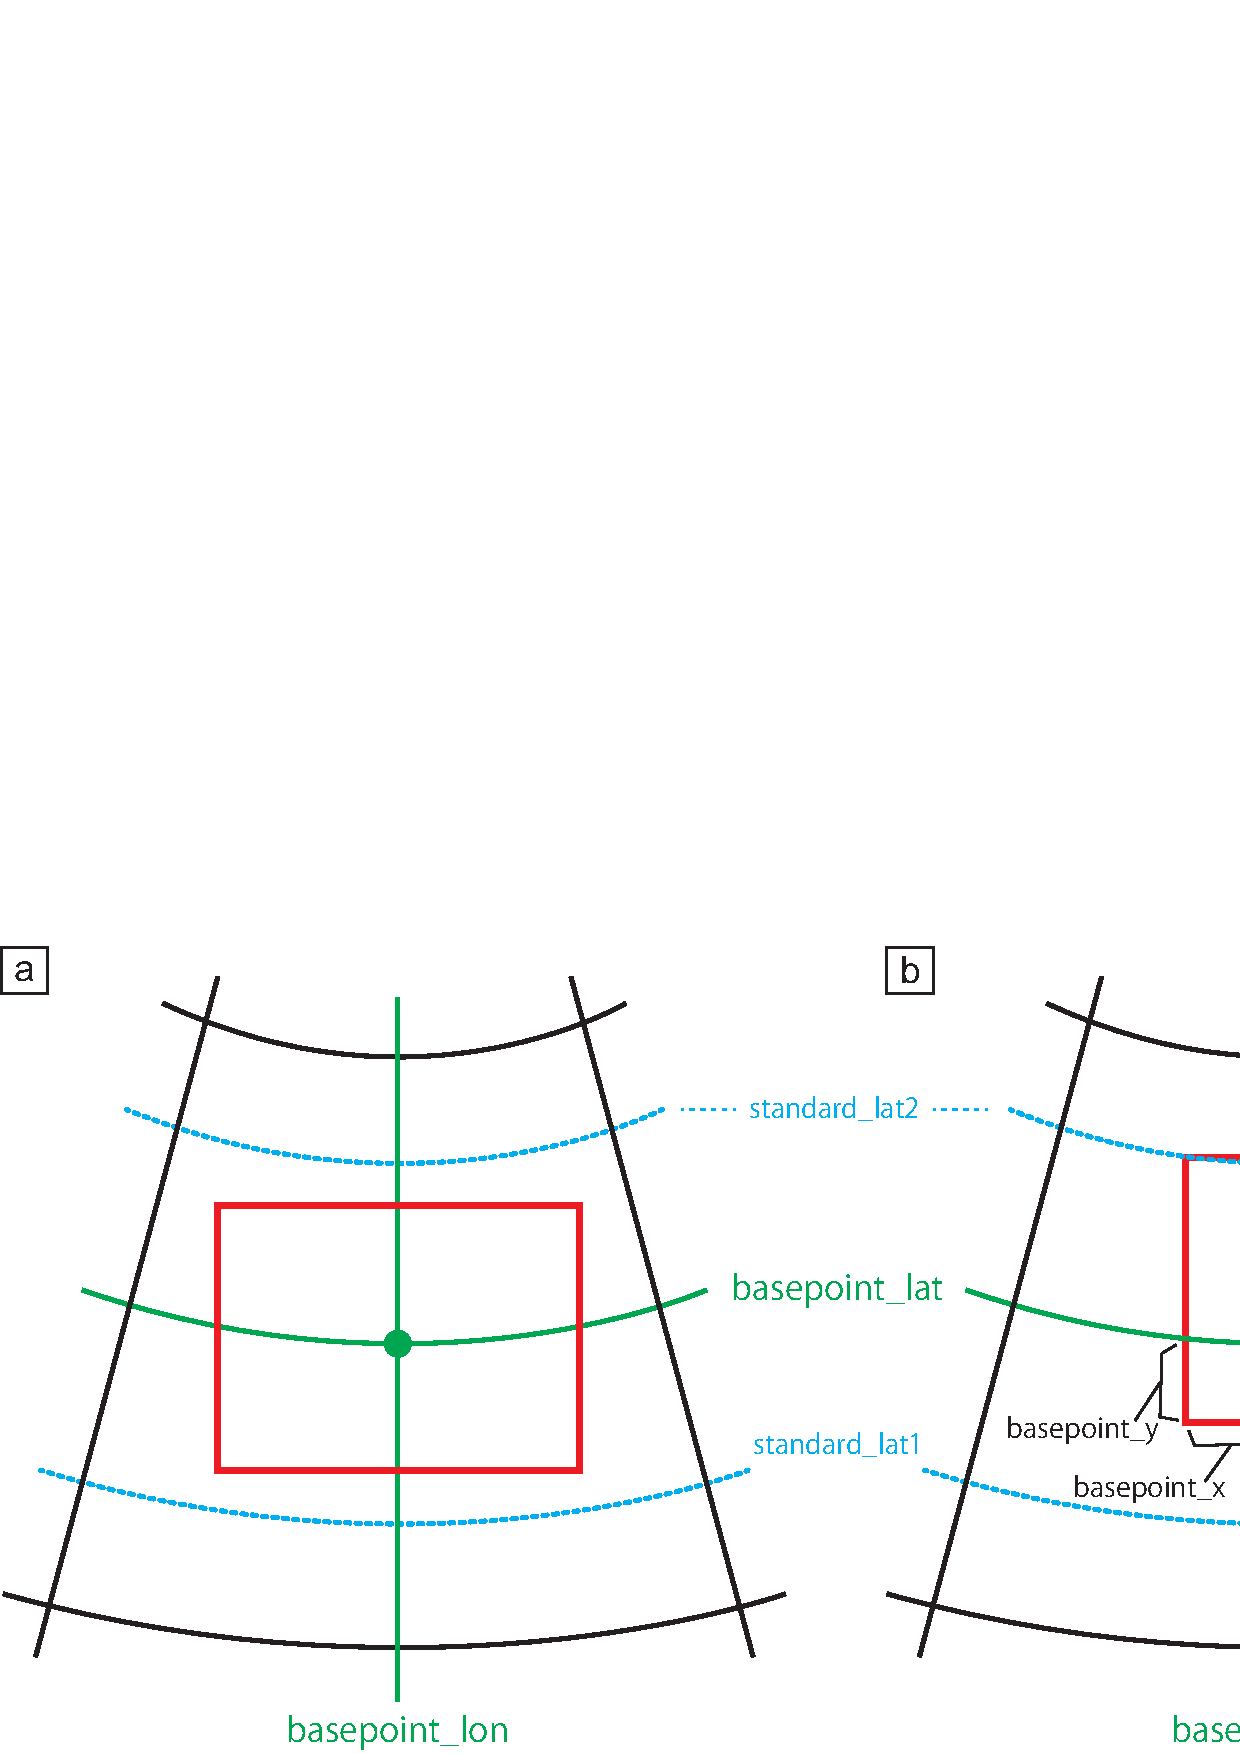
\includegraphics[width=0.8\hsize]{./../../figure/LC_latlon_xy.pdf}\\
  \caption{投影中心と計算領域の関係:(a)はデフォルト設定の場合、(b)は投影中心の位置を計算領域中心からずらした場合。
  赤線は計算領域の境界を表す。}
  \label{fig:map_lc}
\end{center}
\end{figure}
